\documentclass[lang=cn,newtx,10pt,scheme=chinese]{../../Template/elegantbook}

\title{Intial Draft}
\subtitle{空}

\author{邹文杰}
\institute{无}
\date{2024/10/25}
\version{ElegantBook-4.5}
\bioinfo{自定义}{信息}

\extrainfo{宠辱不惊,闲看庭前花开花落;\\去留无意,漫随天外云卷云舒。}

\setcounter{tocdepth}{3}

\logo{logo-blue.png}
\cover{cover.png}

% 本文档额外使用的宏包和命令
\usepackage{../../Styles/mystyle-cumcmthesis}
\usepackage{subfiles}% 主文件额外引用宏包 尽量置于导言区的最后

\begin{document}

\maketitle

\frontmatter

\tableofcontents

\mainmatter


\chapter{问题1}

\section{螺线方程}

在题目图4中的直角坐标系下,以坐标原点\(O\)为极点建立极坐标系,设图4中的等距螺线\(\varGamma\)的极坐标方程为
\begin{align}\label{1..1}
\varGamma :\rho =a+b\theta.
\end{align}
其中\(\rho\)为极径,\(\theta\)为极角,\(a\),\(b\)均为待定常数.设龙头前把手中心的初始位置\(P_0\)极坐标和直角坐标分别为\((\rho _0,\theta _0)\),\((x_0,y_0)\),记\(d_0(\mathrm{m})\)为图4中等距螺线的螺距,则由题可知
\begin{align}
d_0 = 0.55,\rho _0 = 16d_0 = 8.8,\theta _0 = 16\times 2\pi = 32\pi.
\end{align}
又由图4可知图中等距螺线\(\varGamma\)过原点\(O\)和\((\rho _0,\theta _0)\)点,于是将\((0,0)\)和\((\rho _0,\theta _0)\)代入\eqref{1..1}式解得
\begin{align}
    a = 0,b = \frac{d_0}{2\pi}=\frac{0.55}{2\pi}。
\end{align}
因此,等距螺线\(\varGamma\)的极坐标方程为
\begin{align}
\varGamma :\rho =\frac{d_0}{2\pi}\theta ,(0\leqslant \theta \leqslant 32\pi) .\label{0.1}
\end{align}
再利用
\[\begin{cases}
x=\rho \cos \theta\\
y=\rho \sin \theta\\
\end{cases},\]
得到等距螺线\(\varGamma\)的直角坐标方程为
\begin{align}
\varGamma:\begin{cases}
x=\frac{d_0}{2\pi}\theta \cos \theta\\
y=\frac{d_0}{2\pi}\theta \sin \theta\\
\end{cases},(0\leqslant \theta \leqslant 32\pi) .\label{0.0}
\end{align}

\section{计算龙头前把手中心在各时刻的位置}\label{1.(2)}

设龙头前把手的行进速度为\(v_0\),由题可知\(v_0 = 1(\mathrm{m}\cdot s^{-1})\).记龙头前把手中心在第\(t\)秒时的位置为\(P_0(t)\),\(P_0(t)\)点的极坐标和直角坐标分别为\((\rho _0(t),\theta _0(t))\)和\((x_0(t),y_0(t))\),
则利用第一型曲线积分计算公式可得,曲线\(\wideparen{P_0P_0(t)}\)的长度\(S\)为
\begin{align}
S=\int_{\wideparen{P_0P_0(t)}}{\mathrm{d}s}=\int_{\theta _0(t)}^{\theta _0}{\sqrt{[\rho (\theta )]^2+[\rho ' (\theta )]^2}\mathrm{d}\theta}.\label{1.1}
\end{align}
又由题可知
\begin{align}
S = v_0t.\label{1.2}
\end{align}
联立\eqref{0.1}\eqref{1.1}\eqref{1.2}式解得
\begin{align}
\theta _0(t)\sqrt{\theta _{0}^{2}(t)+1}+\ln (\theta _0(t)+\sqrt{(\theta _0(t))^2+1}) =\theta _0\sqrt{\theta _{0}^{2}+1}+\ln (\theta _0+\sqrt{\theta _{0}^{2}+1}) -\frac{4\pi}{d_0}v_0t .
\end{align}
根据上式,利用Python求解得到当\(t\in \{ 1,2,\cdots ,300 \}\)时,\(P_0(t)\)的极角\(\theta _0(t)\),再将其代入\eqref{0.1}式得到,\(P_0(t)\)的极坐标\((\rho _0(t),\theta _0(t))\)见表1.再利用
\begin{align}
\begin{cases}
x_0(t)=\rho _0(t)\cos \theta _0(t)\\
y_0(t)=\rho _0(t)\sin \theta _0(t)\\
\end{cases},
\end{align}
得到当\(t\in \{ 1,2,\cdots ,300 \}\)时,\(P_0(t)\)的的直角坐标\((x_0(t),y_0(t))\)见表2.

\section{计算板凳龙其余各节板凳的后把手中心在各时刻的位置}

记第\(i\)节板凳的后把手中心在第\(t\)秒时的位置为\(P_{i}(t)\),并设\(P_{i}(t)\)的极坐标和直角坐标分别为\((\rho _{i}(t),\theta _{i}(t))\)和\((x_{i}(t),y_{i}(t))\),再记\(P_{i-1}(t)\)与\(P_{i}(t)\)之间的距离为\(| P_{i-1}(t)P_{i}(t)|(\mathrm{m}) (0\leqslant i\leqslant 223)\).再记第$i$节板凳前把手中心与后把手中心之间的距离为\(l_i(\mathrm{m})(1\leq i\leq 223)\),则由条件可知
\begin{gather}
| P_0(t)P_1(t)| = l_1 = 3.41 - 2\times 0.275 = 2.86;
\\
| P_{i-1}(t)P_{i}(t)| = l_i = 2.2 - 2\times 0.275 = 1.65,2\leqslant i\leqslant 223.
\end{gather}

\subsection{计算第1节板凳的后把手中心在第\(t\)秒时的位置\(P_1(t)\)}\label{2.(1)}

当\(t\in \{ 1,2,\cdots ,300 \}\)时,由极坐标系的两点之间距离公式可得
\begin{align}
l_{1}^{2}=| P_0(t)P_1(t)|^2=(\rho _1(t))^2+(\rho _0(t))^2 - 2\rho _1(t)\rho _0(t)\cos (\theta _0(t)-\theta _1(t)) .\label{2.1} 
\end{align}
又因为板凳龙各把手中心均位于螺线\(\varGamma\)上,所以再结合\eqref{0.0}式可得
\begin{align}
\rho _1(t)=\frac{d_0}{2\pi}\theta _1(t),(0\leqslant \theta _1(t)\leqslant 32\pi) .\label{2.2}
\end{align}
因此联立\eqref{2.1}\eqref{2.2}式可得
\begin{align}
l_{1}^{2}=\frac{d_{0}^{2}}{4\pi ^2}[(\theta _1(t))^2+(\theta _0(t))^2 - 2\theta _1(t)\theta _0(t)\cos (\theta _0(t)-\theta _1(t))] .\label{2.0}
\end{align}
根据上式利用Python求解\(\theta _1(t)\),可能得到多个不同解.不妨设这些为不同的解为\(\alpha _{j}^{1}(t) (j = 1,2,\cdots ,m)\),注意到一定有\(\theta _1(t)>\theta _0(t)\),因此令
\begin{align}
A_1 = \{ \alpha _{j}^{1}(t) |\alpha _{j}^{1}(t) >\theta _0(t),j = 1,2,\cdots ,m \} .
\end{align}
又因为龙头前把手与第1节板凳后把手中心的极角之差一定是最小的,所以
\begin{align}
\theta _1(t)=\underset{\alpha _j(t)\in A_1}{\min}\,\left[ \alpha _{j}^{1}(t)-\theta _0\left( t \right) \right] +\theta _0\left( t \right) .
\end{align}
再将上述求得的\(\theta _1(t)\)代入\eqref{2.2}式就能得到此时\(P_1(t)\)的极坐标\((\rho _1(t),\theta _1(t))\).令\(t\)依次取\(1\),\(2\),\(\cdots\),\(300\),反复进行上述操作就能得到,当\(t\in \{ 1,2,\cdots ,300 \}\)时,\(P_1(t)\)的极坐标\((\rho _1(t),\theta _1(t))\).再利用
\begin{align}
\begin{cases}
x_1(t)=\rho _1(t)\cos \theta _1(t)\\
y_1(t)=\rho _1(t)\sin \theta _1(t)\\
\end{cases},    
\end{align}
得到当\(t\in \{ 1,2,\cdots ,300 \}\)时,\(P_1(t)\)的直角坐标\((x_1(t),y_1(t))\).

\subsection{计算第\(i(2\leqslant i\leqslant 223)\)节板凳的后把手中心在第\(t\)秒时的位置\(P_{i}(t)\)}\label{2.(2)}

当\(i\in \{ 2,3,\cdots ,223 \}\)时,由\eqref{2.(1)}同理可得,当\(t\in \{ 1,2,\cdots ,300 \}\)时,我们有
\begin{gather}
l_{i}^{2}=| P_{i-1}(t)P_{i}(t)|^2=(\rho _{i}(t))^2+(\rho _{i-1}(t))^2 - 2\rho _{i}(t)\rho _{i-1}(t)\cos (\theta _{i-1}(t)-\theta _{i}(t)) .\label{2.2.1}
\\
\rho _{i}(t)=\frac{d_0}{2\pi}\theta _{i}(t),(0\leqslant \theta _{i}(t)\leqslant 32\pi) .\label{2.2.2}
\end{gather}
从而联立\eqref{2.2.1}\eqref{2.2.2}式可得
\begin{align}
l_{i}^{2}=\frac{d_{0}^{2}}{4\pi ^2}[(\theta _{i}(t))^2+(\theta _{i-1}(t))^2 - 2\theta _{i}(t)\theta _{i-1}(t)\cos (\theta _{i-1}(t)-\theta _{i}(t))] .\label{2.0.0}
\end{align}
根据上式利用Python求解\(\theta _{i}(t)\),可能得到多个不同解.不妨设这些为不同的解为\(\alpha _{j}^{i}(t) (j = 1,2,\cdots ,m)\),注意到一定有\(\theta _{i}(t)>\theta _{i-1}(t)\),因此令
\begin{align}
A_i = \{ \alpha _{j}^{i}(t) |\alpha _{j}^{i}(t) >\theta _{i-1}(t),j = 1,2,\cdots ,m \},
\end{align}
又因为第\(i - 1\)个把手与第$i$个把手的极角之差一定是最小的,所以
\begin{align}
\theta _i(t)=\underset{\alpha _{j}^{i}(t)\in A_i}{\min}\left[ \alpha _{j}^{i}\left( t \right) -\theta _{i-1}\left( t \right) \right] +\theta _{i-1}\left( t \right) .  
\end{align}
再将上述求得的\(\theta _i(t)\)代入\eqref{2.2}式就能得到此时\(P_{i}(t)\)的极坐标\((\rho _{i}(t),\theta _{i}(t))\).令\(t\)依次取\(1\),\(2\),\(\cdots\),\(300\),反复进行上述操作就能得到,当\(t\in \{ 1,2,\cdots ,300 \}\)时,\(P_{i}(t)\)的极坐标\((\rho _{i}(t),\theta _{i}(t))\).再利用
\begin{align}
\begin{cases}
x_{i}(t)=\rho _{i}(t)\cos \theta _{i}(t)\\
y_{i}(t)=\rho _{i}(t)\sin \theta _{i}(t)\\
\end{cases}, 
\end{align}
得到当\(t\in \{ 1,2,\cdots ,300 \}\)时,\(P_{i}(t)\)的直角坐标\((x_{i}(t),y_{i}(t))\).

综上所述,令\(i\)依次取\(1\),\(2\),\(\cdots\),\(223\),按照上述\eqref{2.(1)}\eqref{2.(2)}的方式,利用Python不断迭代计算就能得到每秒板凳龙各把手中心的位置直角坐标见表3.

\section{计算板凳龙其余各节板凳的后把手中心在各时刻的速度}

记第\(i(1\leqslant i\leqslant 223)\)节板凳的后把手中心在第\(t\)秒时的速度为\(v_i(t)\).根据\eqref{1.(2)},\eqref{2.(1)},\eqref{2.(2)}得到的第\(i(1\leqslant i\leqslant 223)\)节板凳的后把手中心第\(t\)秒时的位置\(P_{i}(t)\)的极坐标\((\rho _{i}(t),\theta _{i}(t))\),于是当\(i\in \{ 1,2,\cdots ,223 \}\)时,对\eqref{2.0}\eqref{2.0.0}式两边同时对\(t\)求导可得
\begin{align}
\frac{\mathrm{d}\theta _i}{\mathrm{d}t}=\frac{\theta _{i - 1}+\theta _i\cos(\theta _{i - 1}-\theta _i)-\theta _i\theta _{i - 1}\sin(\theta _{i - 1}-\theta _i)}{\theta _i+\theta _i\theta _{i - 1}\sin(\theta _{i - 1}-\theta _i)-\theta _{i - 1}\cos(\theta _{i - 1}-\theta _i)}\cdot \frac{\mathrm{d}\theta _{i - 1}}{\mathrm{d}t}.\label{3.0}
\end{align}
设第\(i(1\leqslant i\leqslant 223)\)节板凳的后把手中心在充分短的时间\(\mathrm{d}t\)内经过的路程微分为\(\mathrm{d}s_i\),又因为各把手中心始终在螺线\(\varGamma\)上,从而各把手的路程微分\(\mathrm{d}s_i\)就是螺线\(\varGamma\)的弧微分,所以利用\eqref{0.1}式及弧微分的计算公式可得
\begin{align}
\mathrm{d}s_i=\sqrt{[\rho (\theta _i)]^2+[\rho \prime (\theta _i)]^2}\mathrm{d}\theta _i=\frac{d_0}{2\pi}\sqrt{{\theta _i}^2+1}\mathrm{d}\theta _i,i\in \{ 1,2,\cdots ,223 \}  
\end{align}
故当\(t\in \{ 1,2,\cdots ,300 \}\)时,由瞬时速度的定义可得
\begin{align}
v_i(t) =\frac{\mathrm{d}s_i}{\mathrm{d}t}=\frac{d_0}{2\pi}\frac{\sqrt{{\theta _i}^2 + 1}\mathrm{d}\theta _i}{\mathrm{d}t}, i\in \{1, 2, \cdots, 223\}. \label{3.1}
\end{align}
联立\eqref{3.0}\eqref{3.1}式得到
\begin{align}
|v_i(t)| &= \left|\frac{d_0}{2\pi}\frac{\sqrt{{\theta _i}^2 + 1}\mathrm{d}\theta _i}{\mathrm{d}t}\right| 
= \frac{|\theta _{i - 1} + \theta _i\cos(\theta _{i - 1} - \theta _i) - \theta _i\theta _{i - 1}\sin(\theta _{i - 1} - \theta _i)|}{|\theta _i + \theta _i\theta _{i - 1}\sin(\theta _{i - 1} - \theta _i) - \theta _{i - 1}\cos(\theta _{i - 1} - \theta _i)|}\sqrt{\frac{1 + {\theta _i}^2}{1 + {\theta _{i - 1}}^2}}\left|\frac{\mathrm{d}\theta _{i - 1}}{\mathrm{d}t}\right| \\
&= \frac{|\theta _{i - 1}(t) + \theta _i\cos(\theta _{i - 1} - \theta _i) - \theta _i\theta _{i - 1}\sin(\theta _{i - 1} - \theta _i)|}{|\theta _i + \theta _i\theta _{i - 1}\sin(\theta _{i - 1} - \theta _i) - \theta _{i - 1}\cos(\theta _{i - 1} - \theta _i)|}\sqrt{\frac{1 + {\theta _i}^2}{1 + {\theta _{i - 1}}^2}}|v_{i - 1}(t)|, i\in \{1, 2, \cdots, 223\}.
\end{align}
其中\(\theta _i = \theta _i(t)\),\(\theta _{i - 1} = \theta _{i - 1}(t)\),\(v_0(t) \equiv 1, \forall t\geqslant 0\).又因为\(v_i(t) (1\leqslant i\leqslant 223)\)均大于\(0\),所以上式可化为
\begin{align}
v_i(t) = \sqrt{\frac{1 + {\theta _i}^2}{1 + {\theta _{i - 1}}^2}}\frac{|\theta _{i - 1} + \theta _i\cos(\theta _{i - 1} - \theta _i) - \theta _i\theta _{i - 1}\sin(\theta _{i - 1} - \theta _i)|}{|\theta _i + \theta _i\theta _{i - 1}\sin(\theta _{i - 1} - \theta _i) - \theta _{i - 1}\cos(\theta _{i - 1} - \theta _i)|}v_{i - 1}(t), i\in \{1, 2, \cdots, 223\},
\end{align}
其中\(\theta _i = \theta _i(t)\),\(\theta _{i - 1} = \theta _{i - 1}(t)\),\(v_0(t) \equiv 1, \forall t\geqslant 0\).
于是根据上式,令\(i\)依次取\(1, 2, \cdots, 223\),再利用Python进行迭代计算,就能得到板凳龙的第\(i(1\leqslant i\leqslant 223)\)节板凳的后把手中心在第\(t\)秒时的速度\(v_i(t)\).
再令\(t\)依次取\(1, 2, \cdots, 300\),反复进行上述操作,就能得到当\(t\in \{1, 2, \cdots, 300\}\)时,板凳龙的第\(i(1\leqslant i\leqslant 223)\)节板凳的后把手中心每秒的速度见表\(7\).



\chapter{问题2}

\section{计算各节板凳四个顶点的坐标}

$\forall t\in \mathbb{N}$,根据\textbf{问题1}求解得到龙头前把手中心、第$i(i=1,2,\cdots,223)$节板凳后把手中心在第$t$秒的直角坐标分别为$(x_0(t),y_0(t))$,$(x_i(t),y_i(t))$.设所有板凳的板宽均为$w$,板凳把手中心离最近的板头距离为$h$,则由条件可知$w=0.3m,h=0.275m$.当第$i(i=1,2,\cdots,223)$节板凳后把手刚盘入螺线(即后把手恰好在初始位置)时,记离原点较远且离$P_i$较近的顶点为$A_i$,再按顺时针方向分别记其余顶点为$B_i,C_i,D_i$.记$A_i,B_i,C_i,D_i$在第$t$秒时的位置分别为$A_i(t),B_i(t),C_i(t),D_i(t)$,其直角坐标分别为$(x_{A_i}(t),y_{A_i}(t)),(x_{B_i}(t),y_{B_i}(t)),(x_{C_i}(t),y_{C_i}(t)),(x_{D_i}(t),y_{D_i}(t))$.于是根据向量垂直坐标变换公式可得,对$\forall i\in {0,1,2,\cdots,222}$,都有
\begin{gather}
\overrightarrow{P_{i+1}\left( t \right) P_i\left( t \right) }=\left( x_i\left( t \right) -x_{i+1}\left( t \right) ,y_i\left( t \right) -y_{i+1}\left( t \right) \right) ,\label{problem-2.1}
\\
\overrightarrow{A_i\left( t \right) D_i\left( t \right) }=\overrightarrow{B_i\left( t \right) C_i\left( t \right) }=\left( -\left[ y_i\left( t \right) -y_{i+1}\left( t \right) \right] ,x_i\left( t \right) -x_{i+1}\left( t \right) \right) ,\label{problem-2.2}
\\
\left| \overrightarrow{A_i\left( t \right) D_i\left( t \right) } \right|=\left| \overrightarrow{B_i\left( t \right) C_i\left( t \right) } \right|=w.\label{problem-2.3}
\end{gather}
再记$B_iC_i$和$A_iD_i$的中点分别为$E_i,F_i$,它们在第$t$秒时的位置分别为$E_i(t),F_i(t)$,直角坐标分别为
\begin{align}
E_i(t)=(x_{E_i}(t),y_{E_i}(t)),
\\
F_i(t)=(x_{F_i}(t),y_{F_i}(t)).
\end{align}
从而
\begin{gather}
\overrightarrow{P_{i+1}\left( t \right) E_i\left( t \right) }=\left( x_{E_i}\left( t \right) -x_{i+1}\left( t \right) ,y_{E_i}\left( t \right) -x_{i+1}\left( t \right) \right) ,\label{problem-2.4}
\\
\overrightarrow{P_i\left( t \right) F_i\left( t \right) }=\left( x_{F_i}\left( t \right) -x_i\left( t \right) ,y_{F_i}\left( t \right) -x_i\left( t \right) \right) ,\label{problem-2.5}
\\
\left| \overrightarrow{P_{i+1}\left( t \right) E_i\left( t \right) } \right|=\left| \overrightarrow{P_i\left( t \right) F_i\left( t \right) } \right|=h.\label{problem-2.6}
\\
\overrightarrow{E_i\left( t \right) B_i\left( t \right) }=\left( x_{B_i}\left( t \right) -x_{E_i}\left( t \right) ,y_{B_i}\left( t \right) -y_{E_i}\left( t \right) \right) ,\label{problem-2..1}
\\
\overrightarrow{E_i\left( t \right) C_i\left( t \right) }=\left( x_{C_i}\left( t \right) -x_{E_i}\left( t \right) ,y_{C_i}\left( t \right) -y_{E_i}\left( t \right) \right) ,\label{problem-2..2}
\\
\overrightarrow{F_i\left( t \right) A_i\left( t \right) }=\left( x_{A_i}\left( t \right) -x_{F_i}\left( t \right) ,y_{A_i}\left( t \right) -y_{F_i}\left( t \right) \right) ,\label{problem-2..3}
\\
\overrightarrow{F_i\left( t \right) D_i\left( t \right) }=\left( x_{D_i}\left( t \right) -x_{F_i}\left( t \right) ,y_{D_i}\left( t \right) -y_{F_i}\left( t \right) \right) .\label{problem-2..4}
\end{gather}
由$E_i,P_i,P_{i+1},F_i$共线可得
\begin{gather}
\overrightarrow{P_{i+1}\left( t \right) E_i\left( t \right) }=-\frac{\overrightarrow{P_{i+1}\left( t \right) P_i\left( t \right) }}{\left| \overrightarrow{P_{i+1}\left( t \right) P_i\left( t \right) } \right|}\cdot \left| \overrightarrow{P_{i+1}\left( t \right) E_i\left( t \right) } \right|,\label{problem-2.7}
\\
\overrightarrow{P_i\left( t \right) F_i\left( t \right) }=\frac{\overrightarrow{P_{i+1}\left( t \right) P_i\left( t \right) }}{\left| \overrightarrow{P_{i+1}\left( t \right) P_i\left( t \right) } \right|}\cdot \left| \overrightarrow{P_{i+1}\left( t \right) E_i\left( t \right) } \right|.\label{problem-2.8}
\end{gather}
联立\eqref{problem-2.1}\eqref{problem-2.4}\eqref{problem-2.5}\eqref{problem-2.6}\eqref{problem-2.7}\eqref{problem-2.8}式可得
\begin{gather}
\begin{cases}
x_{E_i}\left( t \right) =x_{i+1}\left( t \right) -\frac{h}{l_{i+1}}\left( x_i\left( t \right) -x_{i+1}\left( t \right) \right)\\
y_{E_i}\left( t \right) =y_{i+1}\left( t \right) -\frac{h}{l_{i+1}}\left( y_i\left( t \right) -y_{i+1}\left( t \right) \right)\\
\end{cases},\label{problem-2.9}
\\
\begin{cases}
x_{F_i}\left( t \right) =x_i\left( t \right) +\frac{h}{l_{i+1}}\left( x_i\left( t \right) -x_{i+1}\left( t \right) \right)\\
y_{F_i}\left( t \right) =y_i\left( t \right) +\frac{h}{l_{i+1}}\left( y_i\left( t \right) -y_{i+1}\left( t \right) \right)\\
\end{cases}.\label{problem-2.10}
\end{gather}
又由$E_i$是$B_i,C_{i}$的中点和$F_i$是$A_i,D_i$的中点可得
\begin{gather}
\overrightarrow{E_i\left( t \right) B_i\left( t \right) }=-\frac{\overrightarrow{B_i\left( t \right) C_i\left( t \right) }}{2},\label{problem-2.11}
\\
\overrightarrow{E_i\left( t \right) C_i\left( t \right) }=\frac{\overrightarrow{B_i\left( t \right) C_i\left( t \right) }}{2},\label{problem-2.12}
\\
\overrightarrow{F_i\left( t \right) A_i\left( t \right) }=-\frac{\overrightarrow{A_i\left( t \right) D_i\left( t \right) }}{2},\label{problem-2.13}
\\
\overrightarrow{F_i\left( t \right) D_i\left( t \right) }=\frac{\overrightarrow{A_i\left( t \right) D_i\left( t \right) }}{2}.   \label{problem-2.14} 
\end{gather}
因此联立\eqref{problem-2.2}\eqref{problem-2.3}\eqref{problem-2..1}\eqref{problem-2..2}\eqref{problem-2..3}\eqref{problem-2..4}\eqref{problem-2.9}\eqref{problem-2.10}\eqref{problem-2.11}\eqref{problem-2.12}\eqref{problem-2.13}式,解得
\begin{gather}
\begin{cases}
x_{A_i}\left( t \right) =x_i\left( t \right) +\frac{h}{l_{i+1}}\left( x_i\left( t \right) -x_{i+1}\left( t \right) \right) +\frac{y_i\left( t \right) -y_{i+1}\left( t \right)}{2}\\
y_{A_i}\left( t \right) =y_i\left( t \right) +\frac{h}{l_{i+1}}\left( y_i\left( t \right) -y_{i+1}\left( t \right) \right) -\frac{x_i\left( t \right) -x_{i+1}\left( t \right)}{2}\\
\end{cases},
\\
\begin{cases}
x_{B_i}\left( t \right) =x_{i+1}\left( t \right) -\frac{h}{l_{i+1}}\left( x_i\left( t \right) -x_{i+1}\left( t \right) \right) +\frac{y_i\left( t \right) -y_{i+1}\left( t \right)}{2}\\
y_{B_i}\left( t \right) =y_{i+1}\left( t \right) -\frac{h}{l_{i+1}}\left( y_i\left( t \right) -y_{i+1}\left( t \right) \right) -\frac{x_i\left( t \right) -x_{i+1}\left( t \right)}{2}\\
\end{cases},
\\
\begin{cases}
x_{C_i}\left( t \right) =x_{i+1}\left( t \right) -\frac{h}{l_{i+1}}\left( x_i\left( t \right) -x_{i+1}\left( t \right) \right) -\frac{y_i\left( t \right) -y_{i+1}\left( t \right)}{2}\\
y_{C_i}\left( t \right) =y_{i+1}\left( t \right) -\frac{h}{l_{i+1}}\left( y_i\left( t \right) -y_{i+1}\left( t \right) \right) +\frac{x_i\left( t \right) -x_{i+1}\left( t \right)}{2}\\
\end{cases},
\\
\begin{cases}
x_{D_i}\left( t \right) =x_i\left( t \right) +\frac{h}{l_{i+1}}\left( x_i\left( t \right) -x_{i+1}\left( t \right) \right) -\frac{y_i\left( t \right) -y_{i+1}\left( t \right)}{2}\\
y_{D_i}\left( t \right) =y_i\left( t \right) +\frac{h}{l_{i+1}}\left( y_i\left( t \right) -y_{i+1}\left( t \right) \right) +\frac{x_i\left( t \right) -x_{i+1}\left( t \right)}{2}\\
\end{cases}.
\end{gather}

\section{计算板凳龙发生碰撞的时间}

对$\forall t>0$,板凳龙在第$t$秒发生碰撞的充要条件是:当$t=t_0$时,存在$s,k\in \{1,2,\cdots,223\}$,使得$A_s(t),$ $B_s(t),$ $C_s(t),$ $D_s(t)$和$A_k(t)$,$B_k(t)$,$C_k(t)$,$D_k(t)$所对应的两节板凳在第$t$秒发生碰撞,即此时矩形$A_s(t)B_s(t)C_s(t)D_s(t)$和矩形$A_k(t)$ $B_k(t)$ $C_k(t)$ $D_k(t)$有交点.于是我们只需要判断在第$t$秒时,对$\forall i,j\in{1,2,\cdots,223}$,矩形$A_i(t)$ $B_i(t)$ $C_i(t)$ $D_i(t)$和矩形$A_j(t)$ $B_j(t)$ $C_j(t)$ $D_j(t)$是否有交点即可.

\subsection{判断矩形$A_i(t)B_i(t)C_i(t)D_i(t)$和矩形$A_j(t)B_j(t)C_j(t)D_j(t)$是否有交点的算法}\label{判断矩形相交的算法}

任取矩形$A_i(t)B_i(t)C_i(t)D_i(t)$的一条边记为$X_1(t)Y_1(t)$,矩形$A_j(t)B_j(t)C_j(t)D_j(t)$的一条边记为$X_2(t)Y_2(t)$.
则利用向量叉乘的性质(详见\href{https://zhuanlan.zhihu.com/p/644689588}{几何算法:判断两条线段是否相交})可得
\begin{align}
\begin{cases}
\text{若}\left( \overrightarrow{X_1\left( t \right) Y_1\left( t \right) }\times \overrightarrow{X_1\left( t \right) X_2\left( t \right) } \right) \cdot \left( \overrightarrow{X_1\left( t \right) Y_1\left( t \right) }\times \overrightarrow{X_1\left( t \right) Y_2\left( t \right) } \right) >0,\text{则}\overrightarrow{X_1\left( t \right) Y_1\left( t \right) },\overrightarrow{X_2\left( t \right) Y_2\left( t \right) }\text{相交},\\
\text{若}\left( \overrightarrow{X_1\left( t \right) Y_1\left( t \right) }\times \overrightarrow{X_1\left( t \right) X_2\left( t \right) } \right) \cdot \left( \overrightarrow{X_1\left( t \right) Y_1\left( t \right) }\times \overrightarrow{X_1\left( t \right) Y_2\left( t \right) } \right) \leqslant 0,\text{则}\overrightarrow{X_1\left( t \right) Y_1\left( t \right) },\overrightarrow{X_2\left( t \right) Y_2\left( t \right) }\text{不相交}.\\
\end{cases}
\end{align}
将矩形$A_i(t)B_i(t)C_i(t)D_i(t)$和矩形$A_j(t)B_j(t)C_j(t)D_j(t)$的每一条边都代入上式,若所有边代入后都不相交,则这两个矩形无交点,否则有交点.


\subsection{证明板凳龙首次发生碰撞一定是第1节板凳或第2节板凳与其他板凳碰撞}

设板凳龙在第$t$秒首次发生碰撞,假设在第$t$秒第$i(3\leq i\leq 223)$节板凳发生碰撞,不妨设其与第$j(2\leq j<i)$板凳发生碰撞,再设在第$t_1$秒第$j-1$节板凳的前把手中心运动到第$t$秒第$j$节板凳的前把手中心所在位置,注意到$t_1<t$且$1\leq j-1\leq i-1$.若$j-1=1$,则结论显然成立.从而不妨设$2\leq j-1\leq i-1$,则
由于除第1节板凳外,其他板凳的长度都相同,并且每节板凳各把手中心始终沿着螺线$\varGamma$移动,因此由几何关系不难得到,在第$t_1$秒时第$j-1$节板凳的前后把手中心位置与在第$t$秒时第$j$节板凳的前后把手中心位置相同,否则在第$t_1$秒时第$j-1$节板凳必然发生碰撞,这与板凳龙在第$t$秒首次发生碰撞矛盾!同理可得,在第$t_1$秒时第$m$节板凳前后把手中心的位置一定与在第$t$秒时第$m+1$节板凳前后把手中心的位置相同,其中$m=j-1,j-2,\cdots,2$.即
\begin{align}
P_m\left( t \right) =P_{m-1}\left( t_1 \right) ,m=2,3,\cdots ,j.
\end{align}
故第$j-1$节板凳在第$t_1$秒的位置和第$j$节板凳在第$t$秒的位置相同,第$i-1$节板凳在第$t_1$秒的位置和第$i$节板凳在第$t$秒的位置相同.由假设可知第$j-1$节板凳和第$i-1$节板凳在第$t_1$秒一定发生碰撞,这与板凳龙在第$t$秒首次发生碰撞矛盾!故结论成立.


\subsection{判断板凳龙是否发生碰撞}\label{判断板凳龙是否发生碰撞}

在第$t$秒时,若对$\forall i\in\{1,2,\cdots,223\},j=1,2$,将矩形$A_i(t)B_i(t)C_i(t)D_i(t)$和矩形$A_j(t)B_j(t)C_j(t)D_j(t)$代入\eqref{判断矩形相交的算法}后,结果都不相交.则板凳龙在第$t$秒不发生碰撞,否则发生碰撞.

\subsection{计算板凳龙发生碰撞的时间及此时板凳龙各把手的位置和速度}

令$t$依次取$1,2,\cdots$,代入\eqref{判断板凳龙是否发生碰撞},利用Python计算得到板凳龙第一次发生碰撞的时间$t_0$,从而板凳龙盘入的终止时刻为$t_0$.在将$t_0$代入\textbf{问题1}的模型,利用Python求解得到此时板凳龙各把手的位置直角坐标和速度见表.



\chapter{问题3}

根据问题1和问题2,建立优化模型易得.

\chapter{问题4}

\section{证明不可通过改变前后两段调头圆弧半径比例减小调头曲线长度}\label{section4.1}

根据题意,设盘入螺线与盘出螺线与调头区域边界交点分别为$M$和$N$,前一段、后一段调头圆弧圆心分别为$O_1、O_2$.两段圆弧切点为$G$.过点$M$与盘入螺线相切的直线为$l_M$,过点$N$与盘出螺线相切的直线为$l_N$,连接$NG$,$MG$,$O_1M$,$O_1G$,$O_2G$,$O_2N$.
画出板凳龙调头曲线的几何示意图如下:
\begin{figure}[htbp]
\centering
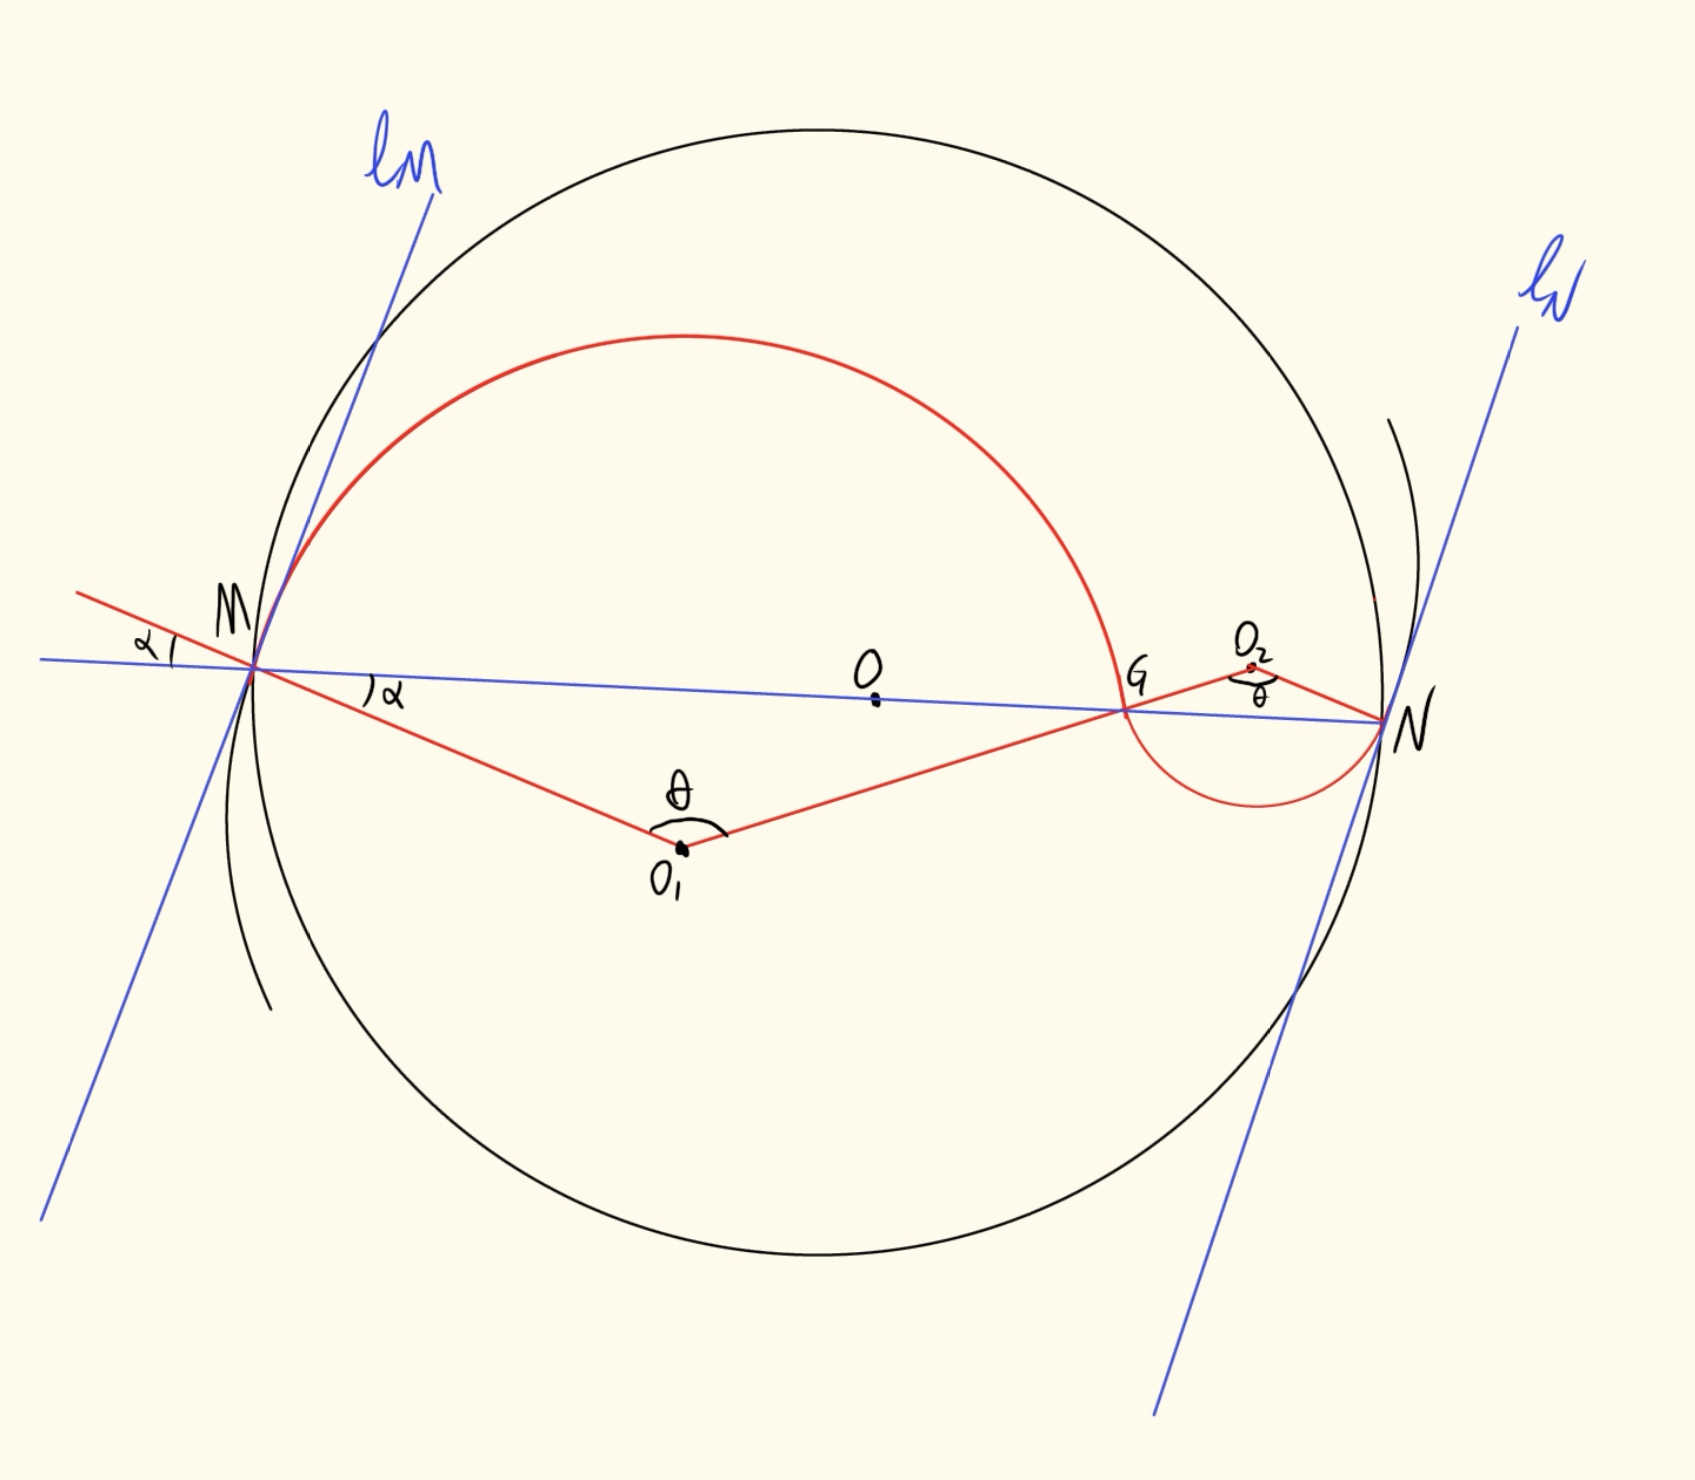
\includegraphics[scale=0.2]{调头曲线示意图.jpg}
\caption{板凳龙调头曲线的几何示意图}
\label{figure1}
\end{figure}
由题可知$O_1,G,O_2$三点共线,从而$\angle MGO_2+\angle O_1GM=\pi .$又注意到$\angle O_1GM=\angle O_2GN$.于是
\begin{align}
\angle MGO_2+\angle O_2GN=\angle MGO_2+\angle O_1GM=\pi .
\end{align}
因此$M,G,N$三点共线.
因为盘入螺线$\varGamma$与盘出螺线$\varGamma'$中心对称,所以$MN$一定过原点$O$且$l_M \varparallel  l_N$.又由$\wideparen{MG}$与$\varGamma$相切,$\wideparen{GN}$与$\varGamma'$相切,可得$O_1M\bot l_M,$ $O_2N\bot l_N$.故$O_1M \varparallel O_2N$.设$\angle MO_1G=\theta$,$\angle O_1MN=\alpha$,则由几何关系易得
\begin{gather}
\angle MO_1G=\angle NO_2G=\theta,
\\
\angle O_1MN=\angle O_1GMN=\angle O_2GN=\angle O_2NG=\alpha .
\end{gather}
设调头区域半径为$R$,则$\left| \overrightarrow{OM} \right|=\left| \overrightarrow{ON} \right|=R$. 设前后两段调头圆弧半径比例为$a:1$,后一段调头圆弧的半径为$r$,则前一段调头圆弧的半径为$ar$,其中$a$为任意常数.则
\begin{align}
\left| \overrightarrow{O_1M} \right|=\left| \overrightarrow{O_1G} \right|=ar,\left| \overrightarrow{O_2N} \right|=\left| \overrightarrow{O_2G} \right|=r.    
\end{align}
设直线$l_M,$ $l_N,$ $O_1M,$ $MN$的斜率分别为$k_{l_M},$ $k_{l_N},$ $k_{O_1M},$ $k_{MN}$.于是根据两直线夹角斜率公式可得
\begin{align}
\tan \alpha =\tan \angle NMO_1=\frac{k_{MN}-k_{l_M}}{1+k_{MN}k_{l_M}}.
\end{align}
从而
\begin{align}
\alpha =\left| \mathrm{arc}\tan \frac{k_{MN}-k_{l_M}}{1+k_{MN}k_{l_M}} \right|.
\end{align}
由$\vartriangle MO_1G\cong \vartriangle NO_2G$可得
\begin{align}
\left| \overrightarrow{NG} \right|=\frac{\left| \overrightarrow{MN} \right|}{1+a}=\frac{2R}{1+a}.
\end{align}
又由几何关系易得
\begin{align}
\theta =\pi -2\alpha ,\quad \cos \alpha =\frac{\frac{1}{2}\left| \overrightarrow{NG} \right|}{\left| \overrightarrow{O_2N} \right|}=\frac{R}{\left( 1+a \right) r}.
\end{align}
因此
\begin{align}
r=\frac{R}{\left( 1+a \right) \cos \alpha}.
\end{align}
设$\wideparen{MG}$的长度为$L_1$,$\wideparen{GN}$的长度为$L_2$,记$L=L_1+L_2$.于是根据圆弧长度计算公式可得
\begin{align}\label{equation-1}
L=L_1+L_2=\theta r+\theta ar=\left( 1+a \right) \theta r=\frac{\left( \pi -2\alpha \right) R}{\cos \alpha}=\frac{\left( \pi -2\left| \mathrm{arc}\tan \frac{k_{MN}-k_{l_M}}{1+k_{MN}k_{l_M}} \right| \right) R}{\cos \left| \mathrm{arc}\tan \frac{k_{MN}-k_{l_M}}{1+k_{MN}k_{l_M}} \right|}.
\end{align}
由上式可知$L$与$a$无关,因此不可通过改变前后两段调头圆弧半径比例减小调头曲线长度.


\section{计算调头曲线长度}

根据题意可知,调头区域边界曲线$S$,盘入螺线$\varGamma$,盘出螺线$\varGamma'$的极坐标方程分别为
\begin{gather}
S:\rho =R,\label{q1}
\\
\varGamma:\rho =\frac{d_0}{2\pi}\theta ,\label{q2}
\\
\varGamma':\rho =-\frac{d_0}{2\pi}\theta.\label{q3}
\end{gather}
于是分别联立\eqref{q1}\eqref{q2}式与\eqref{q1}\eqref{q3}式可分别解出$M,N$的极坐标,分别记为$(\rho_M,\theta_M)$和$(\rho_N,\theta_N)$,则有
\begin{gather}\label{14564}
\begin{cases}
\rho _M=R\\
\theta _M=\frac{2\pi R}{d_0}\\
\end{cases}\quad ,\begin{cases}
\rho _N=R\\
\theta _N=-\frac{2\pi R}{d_0}\\
\end{cases}.
\end{gather}
于是就有
\begin{align}
k_{MN}=k_{OM}=\tan \theta _M=\tan\frac{2\pi R}{d_0}.\label{c1}
\end{align}
又因为$\varGamma$与$\varGamma'$的直角坐标方程分别为
\begin{align}
\varGamma :\begin{cases}
x=\frac{d_0}{2\pi}\theta \cos \theta\\
y=\frac{d_0}{2\pi}\theta \sin \theta\\
\end{cases},\quad \varGamma \prime :\begin{cases}
x=-\frac{d_0}{2\pi}\theta \cos \theta\\
y=-\frac{d_0}{2\pi}\theta \sin \theta\\
\end{cases}
\end{align}
因此我们就有
\begin{gather}
k_{l_M}=\frac{\mathrm{d}y}{dx}\Big |_{M}^{}=\frac{\mathrm{d}y/\mathrm{d}\theta}{dx/\mathrm{d}\theta}\Big |_{M}^{}=\frac{\sin \theta +\theta \cos \theta}{\cos \theta -\theta \sin \theta}\Big |_{\theta =\theta _M}^{},\label{c2}
\\
k_{l_N}=\frac{\mathrm{d}y}{dx}\Big |_{N}^{}=\frac{\mathrm{d}y/\mathrm{d}\theta}{dx/\mathrm{d}\theta}\Big |_{M}^{}=\frac{\sin \theta +\theta \cos \theta}{\cos \theta -\theta \sin \theta}\Big |_{\theta =\theta _M}^{}=\frac{\sin \theta +\theta \cos \theta}{\cos \theta -\theta \sin \theta}\Big | _{\theta =\theta _N}^{}.\label{c3}
\end{gather}
故将\eqref{c1}\eqref{c2}\eqref{c3}代入\eqref{equation-1}计算可得板凳龙的调头曲线长度为
\begin{align}
L=.
\end{align}


\section{计算圆心和切点的坐标}

当前一段圆弧半径是后一段圆弧半径的两倍时,设前一段调头圆弧圆心$O_1$的直角坐标与极坐标分别为$(x_{O_1},y_{O_1})$和$(\rho_{O_1},\theta_{O_1})$,后一段调头圆弧圆心$O_2$的直角坐标为$(x_{O_2},y_{O_2})$和$(\rho_{O_2},\theta_{O_2})$,点$M$的直角坐标为$(x_{M},y_{M})$,点$N$的直角坐标为$(x_{N},y_{N})$,点$G$的直角坐标与极坐标分别为$(x_{G},y_{G})$和$(\rho_{G},\theta_{G})$.
由\eqref{14564}式可得
\begin{align}
\begin{cases}
x_M=\rho _M\cos \theta _M=\\
y_M=\rho _M\sin \theta _M=\\
\end{cases},\quad \begin{cases}
x_N=\rho _N\cos \theta _N=\\
y_N=\rho _N\sin \theta _N=\\
\end{cases}.
\end{align}
根据\eqref{section4.1}的讨论可知
\begin{gather}
\overrightarrow{MG}=2\overrightarrow{GN},
\\
\overrightarrow{MG}=\left( x_G-x_M,y_G-y_M \right) ,
\\
\overrightarrow{GN}=\left( x_N-x_G,y_N-y_G \right) .
\end{gather}
从而
\begin{align}
\begin{cases}
x_G=\frac{x_M+2x_N}{3}=\\
y_G=\frac{y_M+2y_N}{3}=\\
\end{cases}.
\end{align}
于是由几何关系可得
\begin{align}
2R=\left| \overrightarrow{MN} \right|=\left| \overrightarrow{MG} \right|+\left| \overrightarrow{GN} \right|=6r \cos \alpha,
\\
\begin{cases}
\left( x_M-x_{O_1} \right) ^2+\left( y_M-y_{O_1} \right) ^2=4r^2\\
\left( x_G-x_{O_1} \right) ^2+\left( y_G-y_{O_1} \right) ^2=4r^2\\
\end{cases},
\\
\begin{cases}
\left( x_N-x_{O_2} \right) ^2+\left( y_N-y_{O_2} \right) ^2=r^2\\
\left( x_G-x_{O_2} \right) ^2+\left( y_G-y_{O_2} \right) ^2=r^2\\
\end{cases}.
\end{align}
由上式解得
\begin{align}
\begin{cases}
x_{O_1}=\\
y_{O_1}=\\
\end{cases},\quad \begin{cases}
x_{O_2}=\\
y_{O_2}=\\
\end{cases}.
\end{align}
进而得到
\begin{align}
\begin{cases}
\rho _{O_1}=\sqrt{x_{O_1}^{2}+y_{O_1}^{2}}=\\
\theta _{O_1}=\mathrm{arc}\tan \frac{y_{O_1}}{x_{O_1}}=\\
\end{cases},\quad \begin{cases}
\rho _{O_2}=\sqrt{x_{O_2}^{2}+y_{O_2}^{2}}=\\
\theta _{O_2}=\mathrm{arc}\tan \frac{y_{O_2}}{x_{O_2}}=\\
\end{cases}.
\end{align}

\section{计算龙头前把手在各时刻的位置}

\subsection{$P_0$位于盘入螺线$\varGamma$上时}

当$t\in[-100,0]$时,$P_0$位于盘入螺线$\varGamma$上时,我们有
\begin{align}
\left( -t \right) v_0=\int_{\wideparen{P_0M}}{\mathrm{d}s}=\int_{\theta _M}^{\theta _{P_0\left( t \right)}}{\sqrt{\left[ \rho _{\varGamma}\left( \theta \right) \right] ^2+\left[ \rho _{\varGamma}^{\prime}\left( \theta \right) \right] ^2}\mathrm{d}\theta}=\frac{d_0}{2\pi}\int_{\theta _M}^{\theta _{P_0\left( t \right)}}{\sqrt{{\theta}^2+1}\mathrm{d}\theta}.
\end{align}
由上式解得$P_0$的位置坐标.

\subsection{$P_0$位于调头曲线$\wideparen{MG}$上时}

当$t\in[0,\frac{L_1}{v_0}]$时,$P_0$位于调头曲线$\wideparen{MG}$上时,我们有
\begin{gather}
k_{O_1M}=\frac{y_{O_1}-y_M}{x_{O_1}-x_M},k_{O_1P_0\left( t \right)}=\frac{y_{O_1}-y_{P_0\left( t \right)}}{x_{O_1}-x_{P_0\left( t \right)}},
\\
\tan \angle P_0\left( t \right) O_1M=\frac{k_{O_1M}-k_{O_1P_0\left( t \right)}}{1+k_{O_1M}k_{O_1P_0\left( t \right)}}\in \left[ 0,\pi \right] ,
\\
v_0t =\angle P_0\left( t \right) O_1M\cdot 2r,
\\
\left( x_{O_1}-x_{P_0\left( t \right)} \right) ^2+\left( y_{O_1}-y_{P_0\left( t \right)} \right) ^2=4r^2.
\end{gather}
从而
\begin{gather}
\tan \frac{v_0t}{2r}=\tan \angle P_0\left( t \right) O_1M=\frac{k_{O_1M}-k_{O_1P_0\left( t \right)}}{1+k_{O_1M}k_{O_1P_0\left( t \right)}}=\frac{\frac{y_{O_1}-y_M}{x_{O_1}-x_M}-\frac{y_{O_1}-y_{P_0\left( t \right)}}{x_{O_1}-x_{P_0\left( t \right)}}}{1+\frac{y_{O_1}-y_M}{x_{O_1}-x_M}\frac{y_{O_1}-y_{P_0\left( t \right)}}{x_{O_1}-x_{P_0\left( t \right)}}},
\\
\left( x_{O_1}-x_{P_0\left( t \right)} \right) ^2+\left( y_{O_1}-y_{P_0\left( t \right)} \right) ^2=4r^2.
\end{gather}
由上式解得$P_0$的位置坐标.

\subsection{$P_0$位于调头曲线$\wideparen{GN}$上时}

当$t\in[\frac{L_1}{v_0},\frac{L}{v_0}]$时,$P_0$位于调头曲线$\wideparen{GN}$上时,我们有
\begin{gather}
k_{O_2G}=\frac{y_{O_2}-y_G}{x_{O_2}-x_G},k_{O_2P_0\left( t \right)}=\frac{y_{O_2}-y_{P_0\left( t \right)}}{x_{O_2}-x_{P_0\left( t \right)}},
\\
\tan \angle P_0\left( t \right) O_2G=\frac{k_{O_2G}-k_{O_2P_0\left( t \right)}}{1+k_{O_2G}k_{O_2P_0\left( t \right)}}\in \left[ 0,\pi \right] ,
\\
v_0\left( t-\frac{L_1}{v_0} \right) =\angle P_0\left( t \right) O_2G\cdot r,
\\
\left( x_{O_2}-x_{P_0\left( t \right)} \right) ^2+\left( y_{O_2}-y_{P_0\left( t \right)} \right) ^2=r^2.
\end{gather}
从而
\begin{gather}
\tan \frac{v_0\left( t-\frac{L_1}{v_0} \right)}{r}=\tan \angle P_0\left( t \right) O_2G=\frac{k_{O_2G}-k_{O_2P_0\left( t \right)}}{1+k_{O_2G}k_{O_2P_0\left( t \right)}}=\frac{\frac{y_{O_2}-y_G}{x_{O_2}-x_G}-\frac{y_{O_2}-y_{P_0\left( t \right)}}{x_{O_2}-x_{P_0\left( t \right)}}}{1+\frac{y_{O_2}-y_G}{x_{O_2}-x_G}\frac{y_{O_2}-y_{P_0\left( t \right)}}{x_{O_2}-x_{P_0\left( t \right)}}},
\\
\left( x_{O_2}-x_{P_0\left( t \right)} \right) ^2+\left( y_{O_2}-y_{P_0\left( t \right)} \right) ^2=r^2.
\end{gather}
由上式解得$P_0$的位置坐标.

\subsection{$P_0$位于盘出螺线$\varGamma'$上时}

当$t\in[\frac{L}{v_0},100]$时,$P_0$位于盘出螺线$\varGamma'$上时,我们有
\begin{align}
v_0\left( t-\frac{L}{v_0} \right) =\int_{P_0\left( t \right) N}{\mathrm{d}s}=\int_{\theta _N}^{\theta _{P_0\left( t \right)}}{\sqrt{\left[ \rho _{\varGamma \prime}\left( \theta \right) \right] ^2+\left[ \rho _{\varGamma \prime}^{\prime}\left( \theta \right) \right] ^2}\mathrm{d}\theta}=\frac{d_0}{2\pi}\int_{\theta _N}^{\theta _{P_0\left( t \right)}}{\sqrt{\left( \theta +1 \right) ^2+1}\mathrm{d}\theta }.
\end{align}
即
\begin{align*}
v_0\left( t-\frac{L}{v_0} \right) =\frac{d_0}{4\pi}\left[ \theta _{P_0}(t)\sqrt{\left( \theta _{P_0}(t) \right) ^2+1}-\theta _N\sqrt{\theta _{N}^{2}+1}+\ln \left( \theta _{P_0}(t)+\sqrt{\left( \theta _{P_0}(t) \right) ^2+1} \right) -\ln \left( \theta _N+\sqrt{\theta _{N}^{2}+1} \right) \right] .
\end{align*}
由上式解得$P_0$的位置坐标.

\section{计算板凳龙从-100s到100s各把手的位置}

当$t\in[-100,100]$时,板凳龙部分把手位于调头曲线上,此时需要对板凳龙的运动轨迹分段处理,我们将板凳龙的运动轨迹分为盘入螺线$\varGamma$、前一段调头曲线$\wideparen{MG}$、后一段调头曲线$\wideparen{GN}$、盘出螺线$\varGamma'$四段.
然后我们需要根据前一个把手的位置判断与其相邻的后一个把手所在的轨迹曲线,进而递推解出后一个把手的位置.

\subsection{情形一}

当第$t$秒$P_i(0\leq i\leq 222)$在盘入螺线$\varGamma$上时,利用问题1的模型求解$P_{i+1}$的直角坐标即可.

\subsection{情形二}

\subsubsection{引入判断角$\beta_1$}

当第$t$秒$P_i(0\leq i\leq 222)$在$\wideparen{MG}$上时,引入判断角.若$P_{i+1}$与$M$点重合,则定义此时$\angle P_iO_1P_{i+1}=\beta_1$,称$\beta_1$为$\wideparen{MG}$判断角. 几何示意图如下:
\begin{figure}[htbp]
\centering
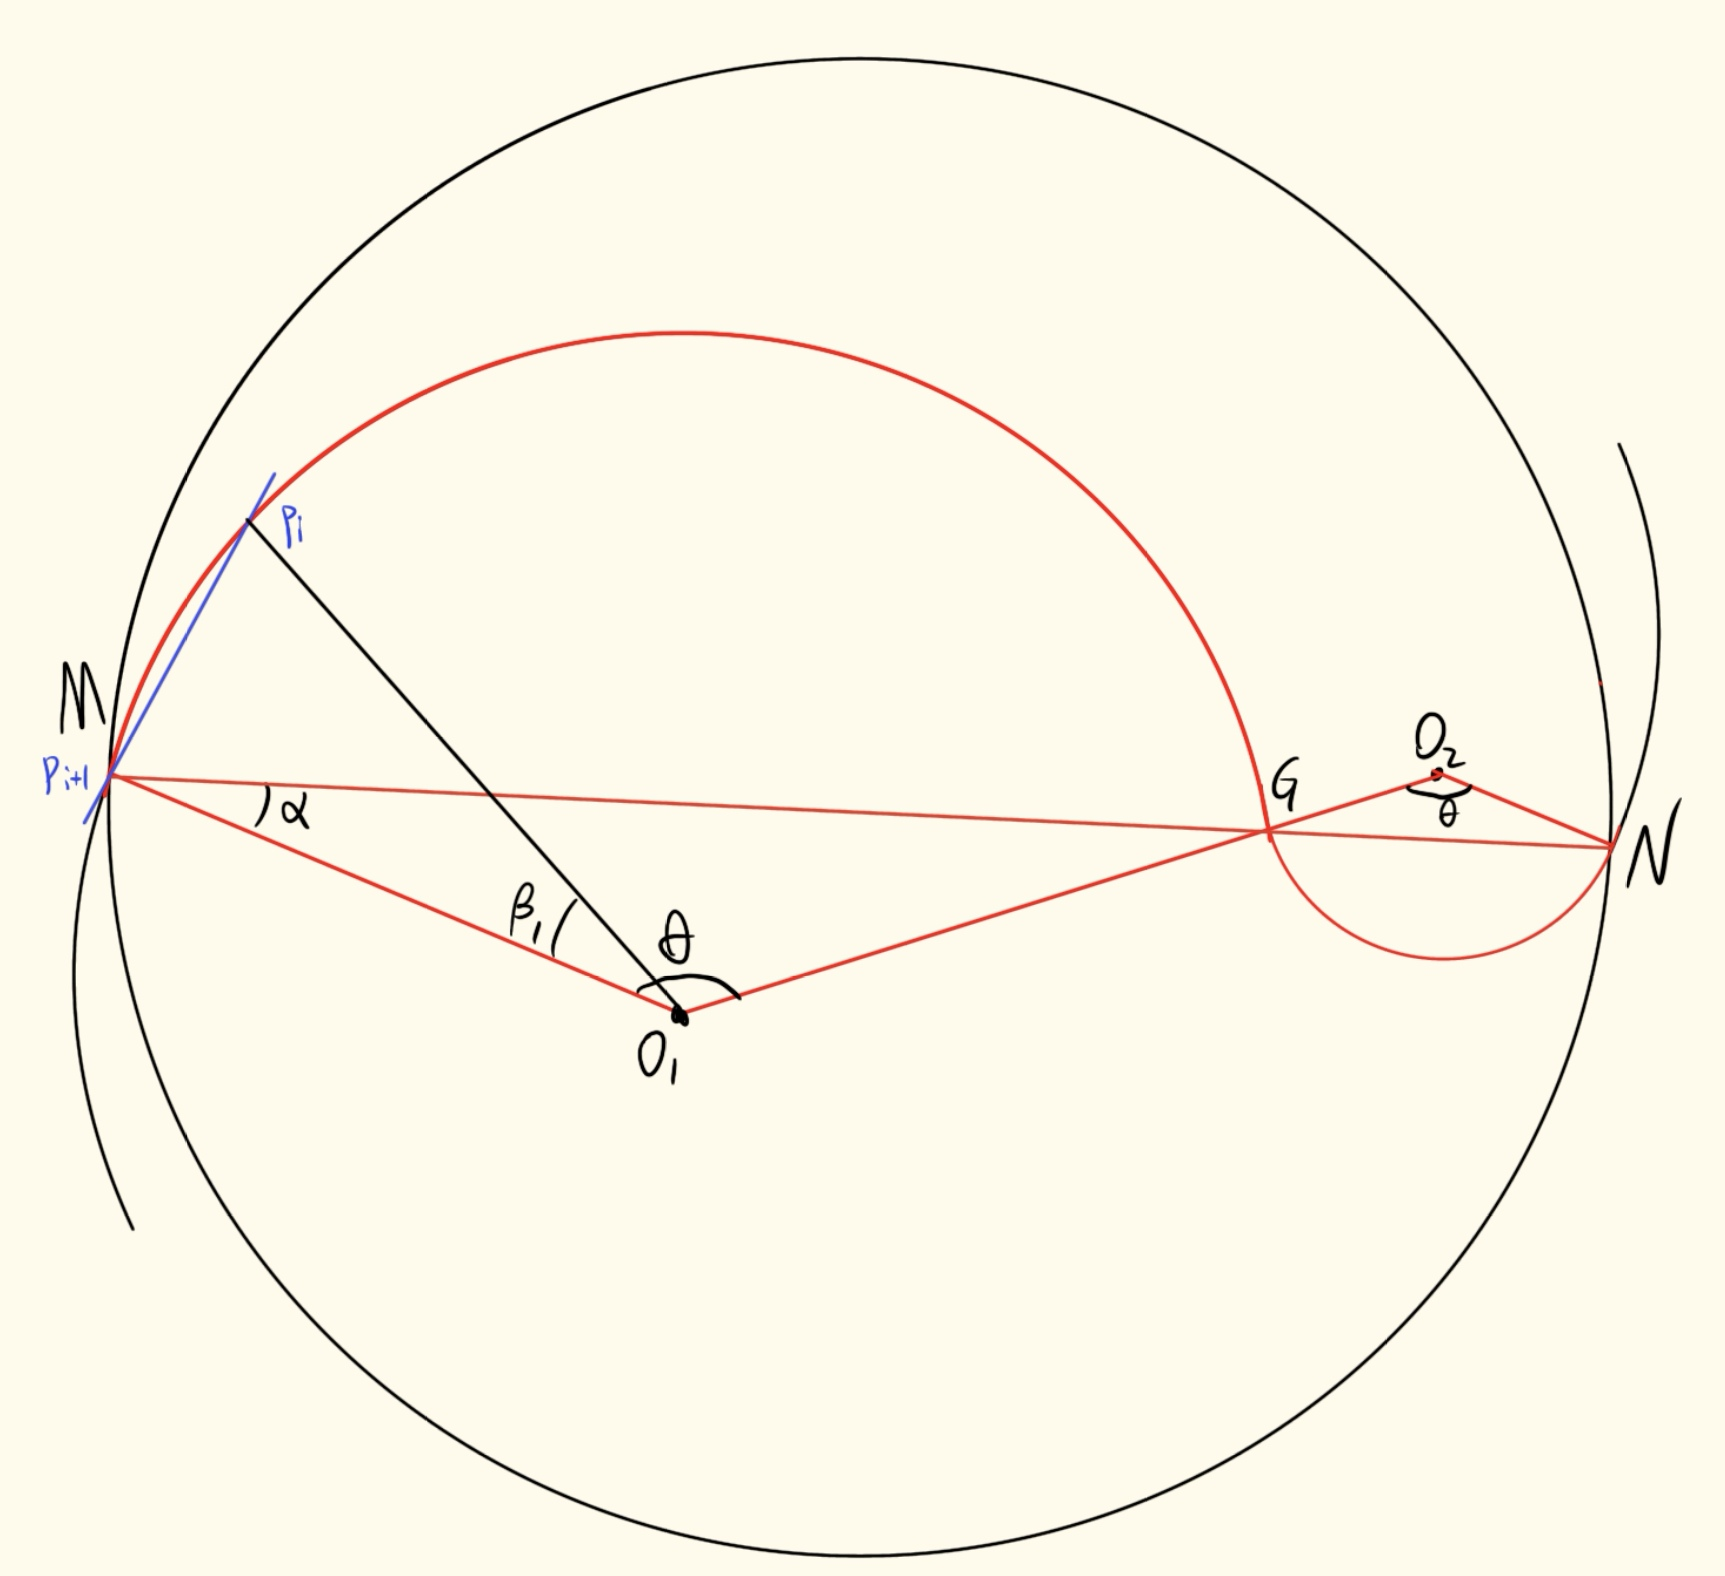
\includegraphics[scale=0.2]{几何示意图1.jpg}
\caption{几何示意图1}
\label{figure2}
\end{figure}
此时由余弦定理可得
\begin{align}
l_{i+1}^{2}=\left| \overrightarrow{P_iP_{i+1}} \right|^2=4r^2-4r^2\cos \beta _1.
\end{align}
由上式解得
\begin{align}
\beta _1=\left| \mathrm{arc}\cos \left( 1-\frac{l_{i+1}^{2}}{4r^2} \right) \right|=.
\end{align}

\subsubsection{计算$\angle P_{i}(t)O_1M$}

根据几何关系及两直线夹角斜率公式可得
\begin{gather}
k_{O_1M}=\frac{y_M-y_{O_1}}{x_M-x_{O_1}},k_{O_1P_i\left( t \right)}=\frac{y_{P_i\left( t \right)}-y_{O_1}}{x_{P_i\left( t \right)}-x_{O_1}},
\\
\tan \angle P_i(t)O_1M=\frac{k_{O_1M}-k_{O_1P_i\left( t \right)}}{1+k_{O_1M}k_{O_1P_i\left( t \right)}}.
\end{gather}
从而
\begin{align}
\angle P_i(t)O_1M= \mathrm{arc}\tan \frac{\frac{y_M-y_{O_1}}{x_M-x_{O_1}}-\frac{y_{P_i\left( t \right)}-y_{O_1}}{x_{P_i\left( t \right)}-x_{O_1}}}{1+\frac{y_M-y_{O_1}}{x_M-x_{O_1}}\cdot \frac{y_{P_i\left( t \right)}-y_{O_1}}{x_{P_i\left( t \right)}-x_{O_1}}}\in[0,\pi].
\end{align}


\subsubsection{判断并计算$P_{i+1}$的位置}\label{subsubsection4.4.1.2}

若$\angle P_i(t)O_1M\geq \beta_1$,则$P_{i+1}$一定位于圆弧$\wideparen{MG}$上.从而根据几何关系可得
\begin{align}
\left\{ \begin{array}{c}
\left( x_{i+1}-x_i \right) ^2+\left( y_{i+1}-y_i \right) ^2=l_{i+1}^{2}\\
\left( x_{i+1}-x_{O_1} \right) ^2+\left( y_{i+1}-y_{O_1} \right) ^2=4r^2\\
\end{array} \right. .
\end{align}
联立解得$(x_{i+1},y_{i+1})$的多个可能解,结合题意可知,$x_{i+1}$的真实解一定是其中最小的一个.于是就能得到$P_{i+1}$的直角坐标$(x_{i+1},y_{i+1})$.

若$\angle P_i(t)O_1M< \beta_1$,则$P_{i+1}$一定位于盘入螺线$\varGamma$上.从而利用问题1解出$(x_{i+1},y_{i+1})$即可.

\subsection{情形三}

\subsubsection{引入判断角$\beta_2$}

当第$t$秒$P_i(0\leq i\leq 222)$在$\wideparen{GN}$上时,引入判断角.若$P_{i+1}$与$G$点重合,则定义此时$\angle P_iO_1P_{i+1}=\beta_2$,称$\beta_2$为$\wideparen{GN}$判断角. 几何示意图如下:
\begin{figure}[htbp]
\centering
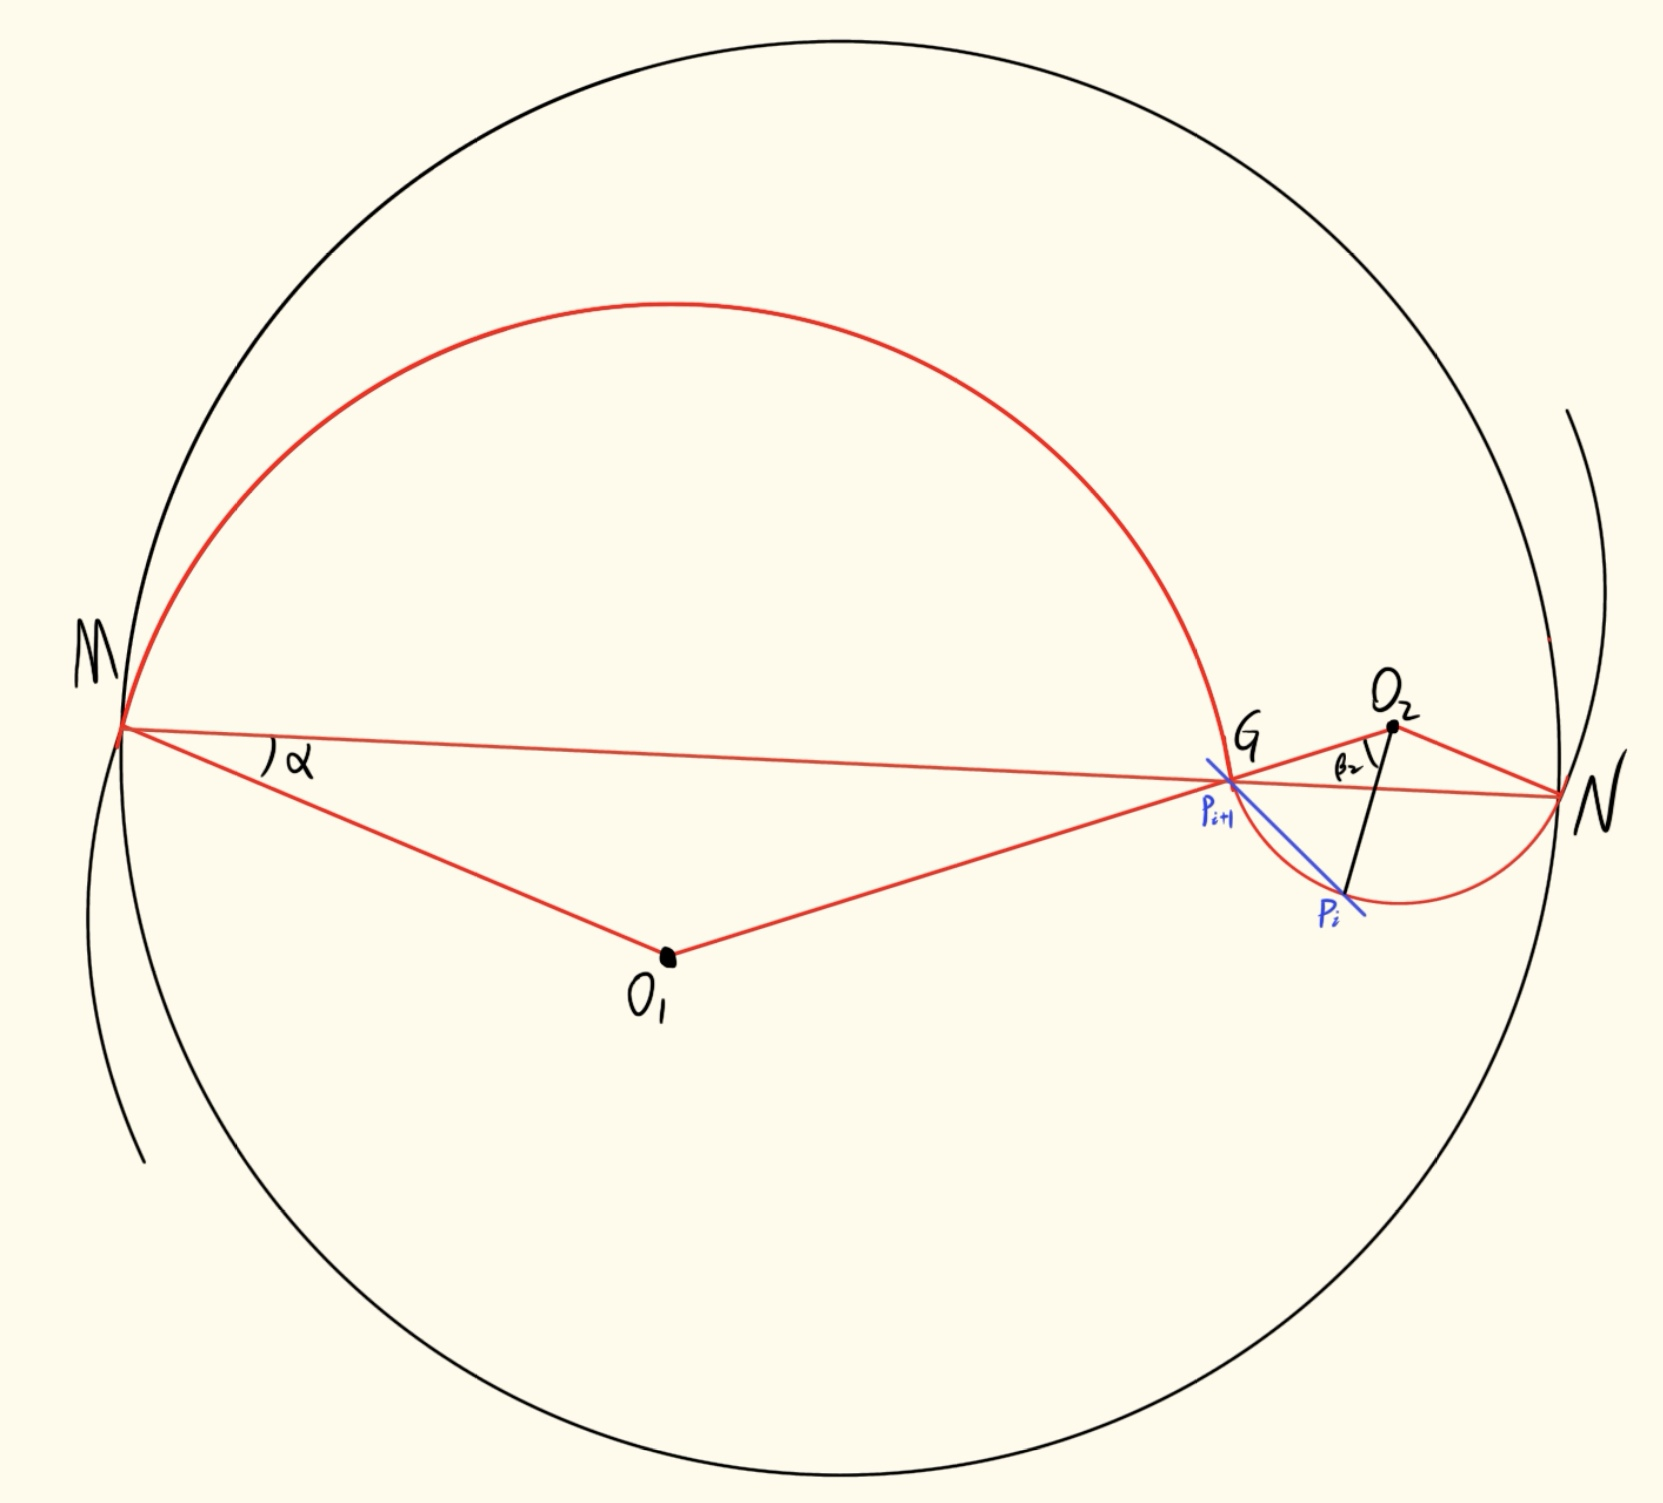
\includegraphics[scale=0.2]{几何示意图2.jpg}
\caption{几何示意图2}
\label{figure3}
\end{figure}
此时由余弦定理可得
\begin{align}
l_{i+1}^{2}=\left| \overrightarrow{P_iP_{i+1}} \right|^2=2r^2-2r^2\cos \beta _2.
\end{align}
由上式解得
\begin{align}
\beta _1=\left| \mathrm{arc}\cos \left( 1-\frac{l_{i+1}^{2}}{2R^2} \right) \right|=.
\end{align}


\subsubsection{计算$\angle P_{i}(t)O_2G$}

根据几何关系及两直线夹角斜率公式可得
\begin{gather}
k_{O_1O_2}=\frac{y_{O_2}-y_{O_1}}{x_{O_2}-x_{O_1}},k_{O_2P_i\left( t \right)}=\frac{y_{P_i\left( t \right)}-y_{O_2}}{x_{P_i\left( t \right)}-x_{O_2}},
\\
\tan \angle P_i(t)O_2G=\frac{k_{O_1O_2}-k_{O_2P_i\left( t \right)}}{1+k_{O_1O_2}k_{O_2P_i\left( t \right)}}.
\end{gather}
从而
\begin{align}
\angle P_i(t)O_2G=\mathrm{arc}\tan \frac{\frac{y_{O_2}-y_{O_1}}{x_{O_2}-x_{O_1}}-\frac{y_{P_i\left( t \right)}-y_{O_2}}{x_{P_i\left( t \right)}-x_{O_2}}}{1+\frac{y_{O_2}-y_{O_1}}{x_{O_2}-x_{O_1}}\frac{y_{P_i\left( t \right)}-y_{O_2}}{x_{P_i\left( t \right)}-x_{O_2}}}\in[0,\pi].
\end{align}


\subsubsection{判断并计算$P_{i+1}$的位置}

若$\angle P_i(t)O_2G\geq \beta_2$,则$P_{i+1}$一定位于圆弧$\wideparen{GN}$上.从而根据几何关系可得
\begin{align}
\left\{ \begin{array}{c}
\left( x_{i+1}-x_i \right) ^2+\left( y_{i+1}-y_i \right) ^2=l_{i+1}^{2}\\
\left( x_{i+1}-x_{O_2} \right) ^2+\left( y_{i+1}-y_{O_2} \right) ^2=r^2\\
\end{array} \right. .
\end{align}
联立解得$(x_{i+1},y_{i+1})$的多个可能解,结合题意可知,$x_{i+1}$的真实解一定是其中最小的一个.于是就能得到$P_{i+1}$的直角坐标$(x_{i+1},y_{i+1})$.

若$\angle P_i(t)O_2G< \beta_2$,则$P_{i+1}$一定位于圆弧$\wideparen{MG}$上.从而利用\eqref{subsubsection4.4.1.2}解出$(x_{i+1},y_{i+1})$即可.

\subsection{情形四}

\subsubsection{引入判断角$\beta_3$}

当第$t$秒$P_i(0\leq i\leq 222)$在$、\varGamma'$上时,引入判断角.若$P_{i+1}$与$N$点重合,则定义此时$\angle P_iO_2N=\beta_3$,称$\beta_3$为$\varGamma'$判断角. 几何示意图如下:
\begin{figure}[htbp]
\centering
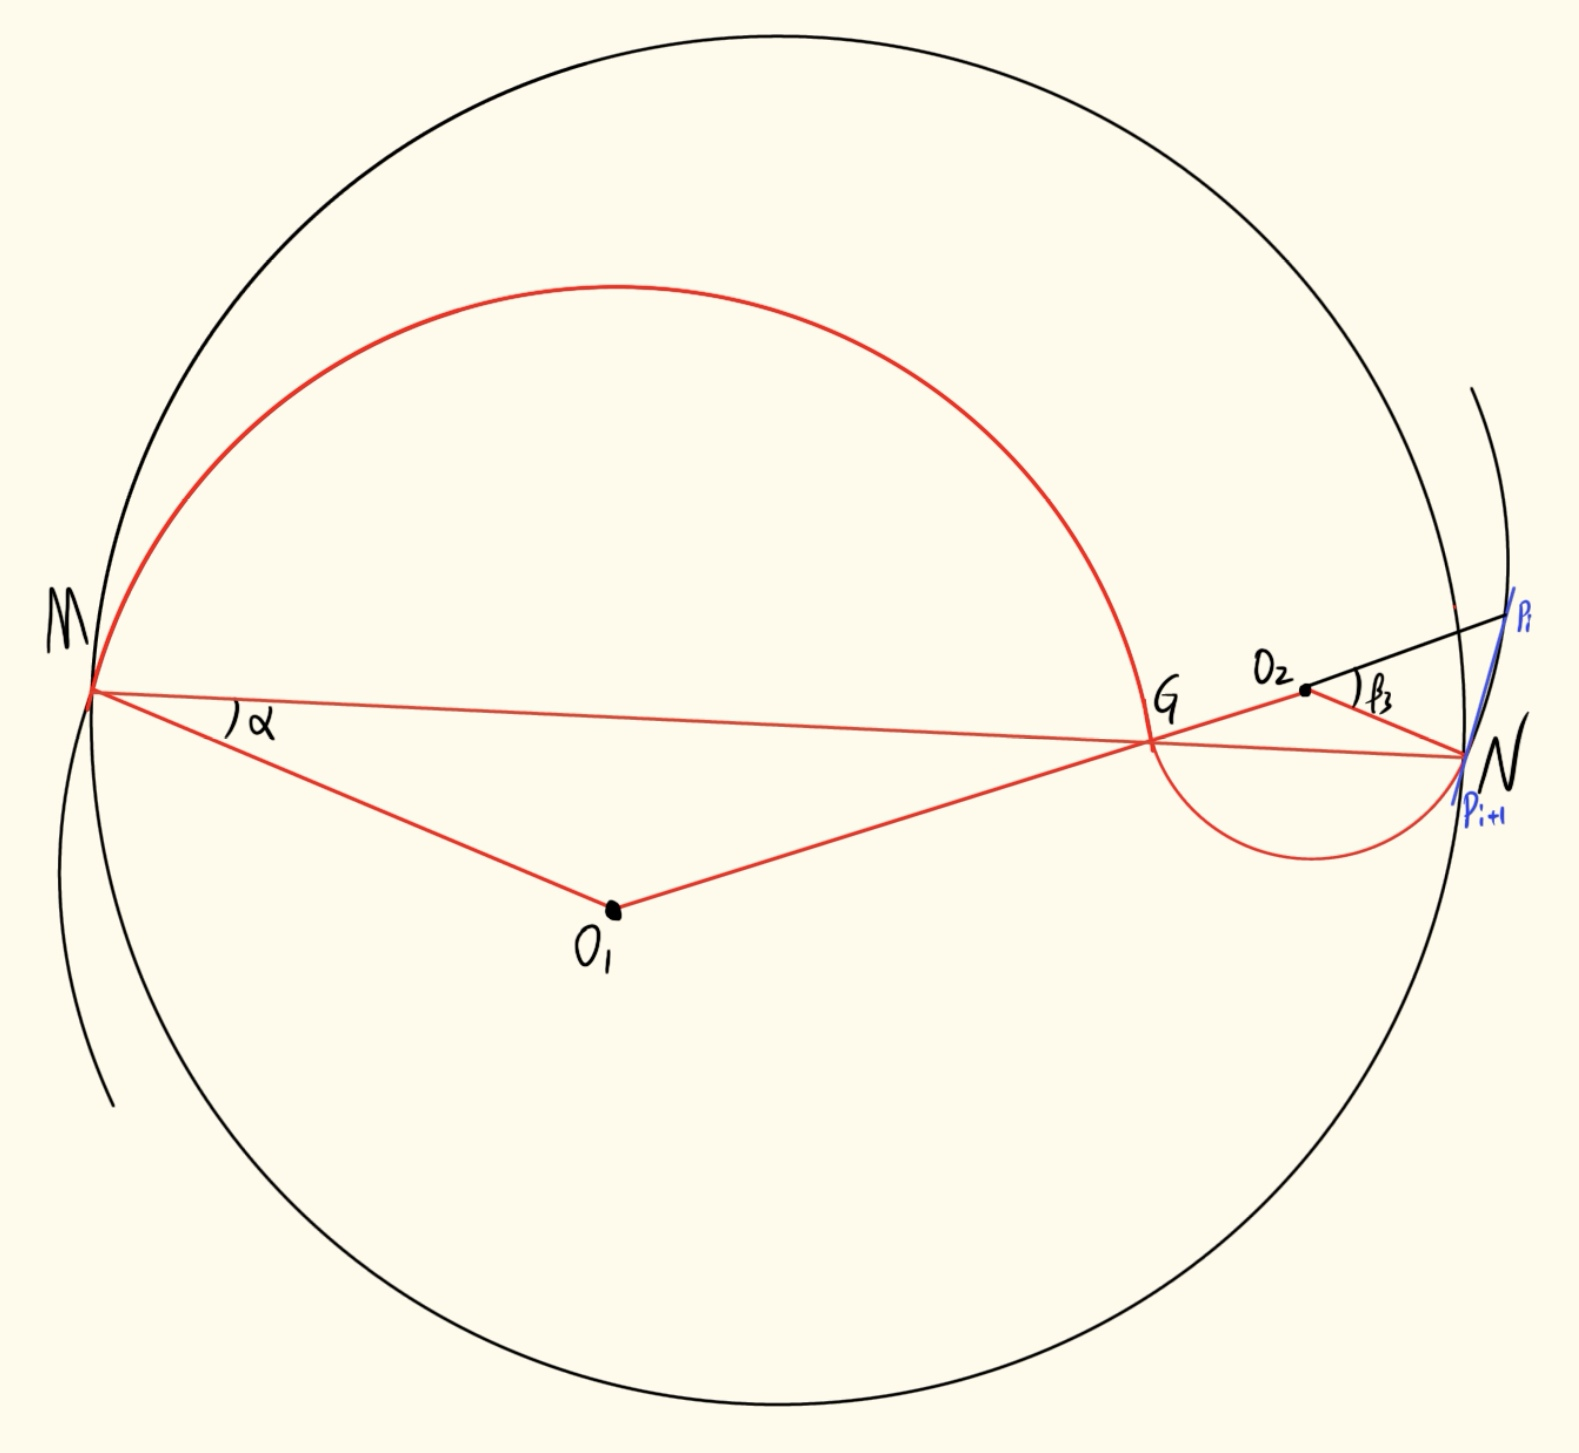
\includegraphics[scale=0.2]{几何示意图3.jpg}
\caption{几何示意图3}
\label{figure4}
\end{figure}
此时由余弦定理可得
\begin{gather}
\left| \overrightarrow{O_2P_i} \right|=\sqrt{\left( x_{P_i}-x_{O_2} \right) ^2+\left( y_{P_i}-y_{O_2} \right) ^2},
\\
l_{i+1}^{2}=\left| \overrightarrow{P_iP_{i+1}} \right|^2=\left| \overrightarrow{O_2P_i} \right|^2+r^2-2r\left| \overrightarrow{O_2P_i} \right|\cos \beta _2.
\end{gather}
由上式解得
\begin{align}
\beta _2=\left| \mathrm{arc}\cos \frac{r^2+\left( x_{P_i}-x_{O_2} \right) ^2+\left( y_{P_i}-y_{O_2} \right) ^2-l_{i+1}^{2}}{2r\sqrt{\left( x_{P_i}-x_{O_2} \right) ^2+\left( y_{P_i}-y_{O_2} \right) ^2}} \right|=.
\end{align}


\subsubsection{计算$\angle P_{i}(t)O_2N$}

根据几何关系及两直线夹角斜率公式可得
\begin{gather}
k_{O_2N}=\frac{y_{O_2}-y_N}{x_{O_2}-x_N},k_{O_2P_i\left( t \right)}=\frac{y_{P_i\left( t \right)}-y_{O_2}}{x_{P_i\left( t \right)}-x_{O_2}},
\\
\tan \angle P_i(t)O_2N=\frac{k_{O_2N}-k_{O_2P_i\left( t \right)}}{1+k_{O_2N}k_{O_2P_i\left( t \right)}}.
\end{gather}
从而
\begin{align}
\angle P_i(t)O_2N=\mathrm{arc}\tan \frac{\frac{y_{O_2}-y_N}{x_{O_2}-x_N}-\frac{y_{P_i\left( t \right)}-y_{O_2}}{x_{P_i\left( t \right)}-x_{O_2}}}{1+\frac{y_{O_2}-y_N}{x_{O_2}-x_N}\frac{y_{P_i\left( t \right)}-y_{O_2}}{x_{P_i\left( t \right)}-x_{O_2}}}\in \left[ 0,\pi \right] .
\end{align}


\subsubsection{判断并计算$P_{i+1}$的位置}

若$\angle P_i(t)O_2N\geq \beta_3$,则$P_{i+1}$一定位于盘出螺线$\varGamma'$上.从而根据几何关系可得
\begin{gather}
l_{i+1}^{2}=|P_i(t)P_{i+1}(t)|^2=(\rho _i(t))^2+(\rho _{i+1}(t))^2-2\rho _i(t)\rho _{i+1}(t)\cos\mathrm{(}\theta _i(t)-\theta _{i+1}(t)),
\\
\rho _{i+1}(t)=\frac{d_0}{2\pi}\left( \theta _{i+1}(t)+\pi \right) .
\end{gather}
根据上式利用Python求解\(\theta _{i}(t)\),可能得到多个不同解.不妨设这些为不同的解为\(\alpha _{j}^{i}(t) (j = 1,2,\cdots ,m)\),注意到一定有\(\theta _{i}(t)<\theta _{i-1}(t)\),因此令
\begin{align}
A_i = \{ \alpha _{j}^{i}(t) |\alpha _{j}^{i}(t) <\theta _{i-1}(t),j = 1,2,\cdots ,m \},
\end{align}
又因为第\(i + 1\)个把手与第$i$个把手的极角之差一定是最小的,所以
\begin{align}
\theta _{i+1}(t)=\underset{\alpha _{j}^{i}(t)\in A_i}{\min}\left[ \alpha _{j}^{i}\left( t \right) -\theta _i\left( t \right) \right] +\theta _i\left( t \right) .
\end{align}
再将上述求得的\(\theta _{i+1}(t)\)代入盘入螺线$\varGamma'$方程就能得到此时\(P_{i+1}(t)\)的极坐标\((\rho _{i+1}(t),\theta _{i+1}(t))\).再利用
\begin{align}
\begin{cases}
x_{i+1}(t)=\rho _{i+1}(t)\cos \theta _{i+1}(t)\\
y_{i+1}(t)=\rho _{i+1}(t)\sin \theta _{i+1}(t)\\
\end{cases}, 
\end{align}
就能得到\(P_{i+1}(t)\)的直角坐标\((x_{i+1}(t),y_{i+1}(t))\).

若$\angle P_i(t)O_2N< \beta_3$,则$P_{i+1}$一定位于圆弧$\wideparen{GN}$上.从而利用情形三解出$(x_{i+1},y_{i+1})$即可.



综上,将$P_0$在不同时刻的坐标代入上述四种情形,不断递推就能得到所有把手的位置坐标.

\section{计算板凳龙从-100s到100s各把手的速度}

结合上述计算得到的各节点在各时刻的位置坐标,再利用问题1的模型递推求解即可.



\chapter{问题5}

根据前四问,建立优化模型易得.

\end{document}